\chapter{Exercises}

\section{Clustering}

Open the ``Liver-cirrhosis'' data set from the \widget{Datasets} widget. It represents a sliced liver tissue. As tissues have holes and they also tear during the slicing some parts of the dataset has very low spectral intensities. Let's call these ``background regions''.

\begin{enumerate}
\item Remove background regions from the data set in any way you see fit. You are likely to need some preprocessing. Also clustering, as seen below, could be useful for for this. Try to make it work.

\vspace{-0.2cm}
\begin{figure}[h]
  \centering
  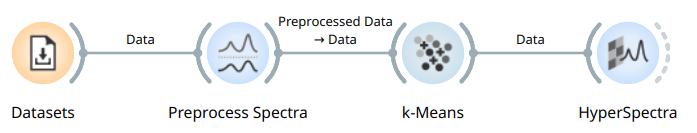
\includegraphics[width=\linewidth]{cirrhosis-background.png}%
  \caption{$\;$}
\end{figure}
\vspace{-0.3cm}

\item Afterwards, find two groups of spectra with the most obvious differences. The preprocessing used for background removal may not be the best for clustering; to obtain a selection of original data, use the \widget{Select by Data Index} widget.

\item Describe differences between the two groups. Try at least \widget{Spectra}, \widget{Distributions}, \widget{Violin Plot}, \widget{Scatter Plot}.

\end{enumerate}


\section{Classification}

\begin{enumerate}

\item Use either a spectral image or unannotated spectra. Manually annotate classes as you see fit. Assign classes only according to shapes in the image or filenames; classes set according to spectral content {\bf will} yield good separation, because that is a tautology.

\item Use Random Forests and Logistic regression. Interpret the models.

\item Observe the effects of different preprocessing on classification performance and model interpretation. Also try models built on the PCA scores.

\end{enumerate}


\section{Game of bias}

Start with a dataset with annotated classes. Randomize class values to destroy connections between spectra and classes. Next, think of a novel way to introduce bias in the data set so that AUC becomes significantly higher than 0.5 even with cross-validation within \widget{Test and Score}.

